\documentclass[12pt,a4paper]{article}

\usepackage{fontawesome5}
\providecommand{\faPencilAlt}{\faIcon{pencil-alt}}

\usepackage{styles/couleurs}
\usepackage{styles/mise_en_page}
\usepackage{styles/boites}
\usepackage{styles/maths}
\usepackage{styles/figures}

\usepackage{enumitem}
\usepackage{array}
\usepackage{tabularx}
\usepackage{amsmath}
\usepackage{amssymb}
\usepackage{tikz}
\usepackage{xparse}
\usepackage{pdflscape}
\usepackage{colortbl}

\usetikzlibrary{calc,arrows.meta,positioning}

\setlist[itemize]{leftmargin=1.4em,itemsep=0.15em,topsep=0.2em}
\setlist[enumerate]{leftmargin=*,itemsep=0.22em,topsep=0.25em}

\newcommand{\lignepointillee}{\noindent\dotfill\par\vspace{0.45em}}

\newcommand{\lignesreponse}[1]{%
\begin{tcolorbox}[
enhanced,colback=white,colframe=NeutreC!40,boxrule=0.5pt,arc=1.5mm,
left=3mm,right=3mm,top=2mm,bottom=1mm,before skip=2pt,after skip=2pt]
\foreach \i in {1,...,#1}{\lignepointillee}
\end{tcolorbox}}

\newcommand{\titreseq}[1]{%
\begin{center}
{\sffamily\LARGE\bfseries\color{TitreC}Séquence 7 -- Arithmétique}\\[0.2em]
{\sffamily\large\bfseries\color{SavoirC}#1}
\end{center}}

\newcommand{\grillecent}{%
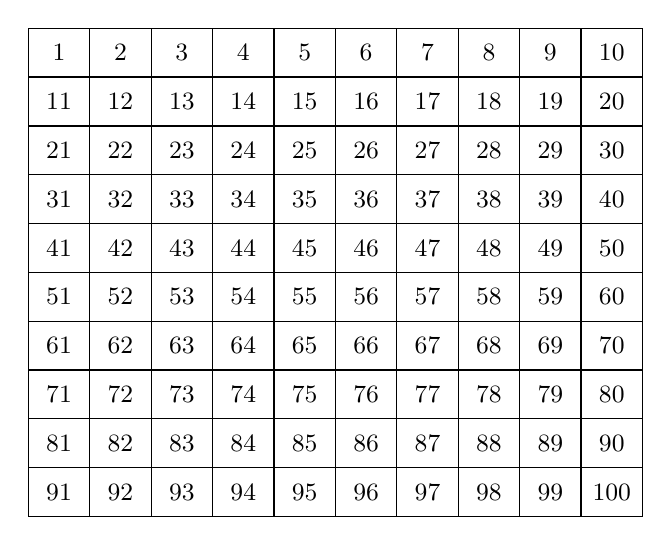
\begin{tikzpicture}[x=0.78cm,y=0.62cm]
  \foreach \n in {1,...,100}{
    \pgfmathtruncatemacro{\col}{mod(\n-1,10)}
    \pgfmathtruncatemacro{\lig}{9-floor((\n-1)/10)}
    \draw[line width=0.45pt] (\col,\lig) rectangle ++(1,1);
    \node[font=\small] at (\col+0.5,\lig+0.5) {\n};
  }
\end{tikzpicture}}

\begin{document}

\titreseq{Progression professeur}

\remarque{Durée indicative : huit séances d'apprentissage de 50 à 55 minutes,
deux interrogations courtes et une évaluation finale.

La séquence distingue explicitement les \textbf{rappels} des apprentissages
nouveaux de 4e.}

\section*{Ce qui relève du rappel}

\begin{itemize}
  \item effectuer et interpréter une division euclidienne ;
  \item utiliser le vocabulaire : multiple, diviseur, divisible ;
  \item dresser une liste de multiples ou de diviseurs ;
  \item utiliser les critères de divisibilité par \(2\), \(3\), \(5\), \(9\) et \(10\) ;
  \item résoudre de petits problèmes de partage ou de rangement.
\end{itemize}

\section*{Ce qui est construit ou consolidé en 4e}

\begin{itemize}
  \item définir et reconnaître un nombre premier ;
  \item connaître la liste des nombres premiers inférieurs à \(100\) ;
  \item décomposer un entier en produit de facteurs premiers ;
  \item reconnaître et produire des fractions égales à l'aide des facteurs premiers ;
  \item simplifier une fraction en supprimant les facteurs communs ;
  \item résoudre des problèmes simples de divisibilité,
        notamment chercher toutes les répartitions possibles.
\end{itemize}

\section*{Ce qui est différé ou laissé en prolongement}

\begin{itemize}
  \item formaliser en 3e la notion de \textbf{fraction irréductible} ;
  \item étendre en 3e la décomposition à de plus grands nombres
        à l'aide d'une calculatrice, d'un tableur ou d'un programme ;
  \item généraliser les tests de primalité à de grands nombres ;
  \item formaliser le nombre de diviseurs à partir des exposants
        d'une décomposition en facteurs premiers ;
  \item n'utiliser le PGCD, le PPCM ou l'algorithme d'Euclide
        que comme enrichissements éventuels, et non comme objectifs centraux
        de cette séquence de 4e.
\end{itemize}

\section*{Objectifs de fin de séquence}

L'élève doit pouvoir :

\begin{itemize}
  \item traduire une situation avec les mots multiple, diviseur et divisible ;
  \item utiliser une division euclidienne ou un critère de divisibilité pour justifier ;
  \item reconnaître un nombre premier et expliquer pourquoi \(1\) ne l'est pas ;
  \item retrouver les nombres premiers inférieurs à \(100\) avec le crible ;
  \item décomposer un nombre en produit de facteurs premiers ;
  \item vérifier une décomposition en effectuant le produit ;
  \item simplifier une fraction grâce aux facteurs communs ;
  \item reconnaître des fractions égales ;
  \item déterminer toutes les possibilités de groupes identiques sans reste ;
  \item rédiger une justification courte et adaptée.
\end{itemize}

\section*{Déroulé réaliste}

\renewcommand{\arraystretch}{1.35}
\begin{tabularx}{\textwidth}{
|>{\centering\arraybackslash}p{1.05cm}
|>{\raggedright\arraybackslash}p{4.2cm}
|>{\raggedright\arraybackslash}X
|>{\raggedright\arraybackslash}p{3cm}|}
\hline
\textbf{Séance} & \textbf{Support principal} &
\textbf{Enjeu didactique} & \textbf{Production}\\
\hline
1 & Activité 1 : l'atelier du menuisier &
Diagnostiquer division euclidienne, quotient, reste et prise en compte
de plusieurs contraintes. & Tableau des ressources et bilan de rappel.\\
\hline
2 & Activité 2 : Juniper Green &
Réactiver multiples et diviseurs dans un jeu ; faire émerger
des nombres ayant très peu de diviseurs. & Stratégie expliquée.\\
\hline
3 & Activité 3 : crible d'Ératosthène &
Construire la liste des nombres premiers inférieurs à \(100\)
et stabiliser la définition. & Grille complétée et liste.\\
\hline
4 & Activité 4 : démonter les nombres &
Faire apparaître qu'une décomposition poursuivie jusqu'aux nombres premiers
aboutit aux mêmes facteurs, quel que soit le chemin. & Arbres de facteurs.\\
\hline
5 & Activité 5 : fractions égales &
Utiliser les facteurs premiers pour reconnaître puis produire
des fractions égales et simplifier. & Interrogation 1 au début.\\
\hline
6 & Activité 6 : bouquets identiques &
Chercher toutes les répartitions possibles par les diviseurs communs,
sans introduire formellement le PGCD. & Tableau de toutes les solutions.\\
\hline
7 & Activité 7 : mission nombres &
Mobiliser critères, primalité, décomposition et raisonnement
dans une activité de synthèse. & Interrogation 2 au début.\\
\hline
8 & Consolidation différenciée &
Automatismes, erreurs fréquentes, problèmes courts et rédaction. &
Préparation de l'évaluation.\\
\hline
9 & Évaluation finale &
Mobiliser rappels, nombres premiers, décomposition, fractions
et problème de partage. & Évaluation sur 20.\\
\hline
\end{tabularx}

\section*{Automatismes}

Rituel de cinq minutes, quatre à six questions :

\begin{itemize}
  \item séances 1 à 3 : multiple, diviseur, reste et critères ;
  \item séances 3 à 5 : premiers ou composés, liste inférieure à \(100\) ;
  \item séances 4 à 7 : décompositions courtes ;
  \item séances 5 à 8 : facteurs communs et simplification de fractions ;
  \item après la séquence : une question de divisibilité ou de décomposition par semaine.
\end{itemize}

\section*{Principes didactiques}

\begin{itemize}
  \item Le vocabulaire est toujours relié à une égalité multiplicative.
  \item Un nombre composé est réfuté en exhibant un diviseur autre que \(1\)
        et lui-même.
  \item Le crible précède la mémorisation de la liste des nombres premiers.
  \item La décomposition est construite par des arbres avant d'être automatisée.
  \item Simplifier une fraction signifie ici enlever des facteurs communs ;
        la terminologie plus formelle est différée.
  \item Les problèmes de groupes identiques sont résolus en donnant
        \textbf{toutes} les possibilités, pas seulement la plus grande.
\end{itemize}

\end{document}
